\documentclass[a4paper]{article}

%% Language and font encodings
\usepackage[english]{babel}
\usepackage[utf8x]{inputenc}
\usepackage[T1]{fontenc}

%% Sets page size and margins
\usepackage[a4paper,top=3cm,bottom=2cm,left=3cm,right=3cm,marginparwidth=1.75cm]{geometry}

%% Useful packages
\usepackage{amsmath}
\usepackage{graphicx}
\usepackage{longtable,tabu}
\usepackage{lipsum}
\usepackage[colorinlistoftodos]{todonotes}
\usepackage[colorlinks=true, allcolors=blue]{hyperref}
\graphicspath{{images/}}

\newcounter{funcreqcounter}
\newenvironment{funcreq}[1][]{
  \begin{quote}
  \renewcommand{\item}{
    \refstepcounter{funcreqcounter}\par
    \textbf{FR\thefuncreqcounter #1} \rmfamily
  }
}{\end{quote}}

\newcounter{seqreqcounter}
\newenvironment{seqreq}[1][]{
  \begin{quote}
  \renewcommand{\item}{
    \refstepcounter{seqreqcounter}\par
    \textbf{SR\theseqreqcounter #1} \rmfamily
  }
}{\end{quote}}

\newcounter{perfreqcounter}
\newenvironment{perfreq}[1][]{
  \begin{quote}
  \renewcommand{\item}{
    \refstepcounter{perfreqcounter}\par
    \textbf{PR\theperfreqcounter #1} \rmfamily
  }
}{\end{quote}}

\title{Disciplina: Requirements Specification}
\author{TeachMePlease, \href{https://teachmeplease.com}{\texttt{https://teachmeplease.com}}}

\date{%
Version 0.1\\%
\today
}

\begin{document}
\maketitle

\section{Introduction}
\subsection{Purpose}
The purpose of this document is to provide a set of formal requirements for the Disciplina platform.

\subsection{Platform description}
Disciplina platform is intended to act like a backend for other educational services. These services include CRM/ERP platforms of educational institutions (e.g., Blackboard, Moodle), online services (e.g., TeachMePlease, Coursera, Khan Academy) and others. The primary goal of the Disciplina platform is to unite all of these diverse sources of educational records and store them in an untamberable ledger. The place of the Disciplina platform in the educational ecosystem is shown in Figure \ref{fig:scope}

\begin{figure}[ht]
  \centering
  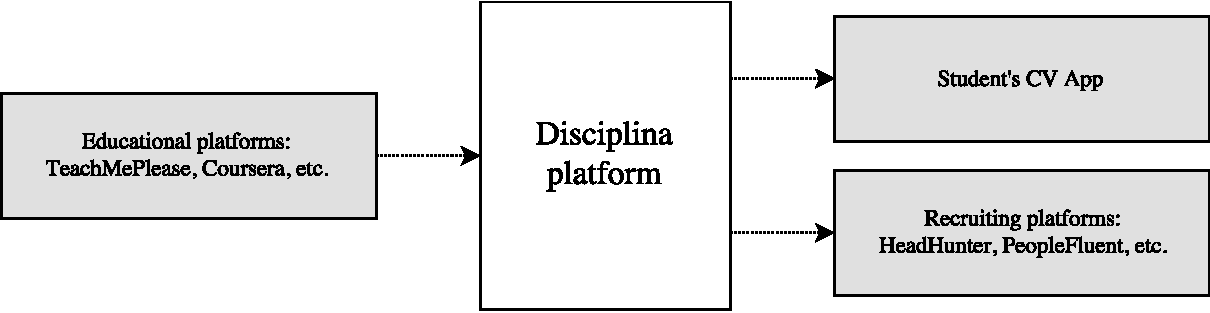
\includegraphics[width=0.8\textwidth]{disciplina-scope}
  \caption{The scope of the Disciplina platform. The arrows denote data flow}
  \label{fig:scope}
\end{figure}

The records that appear during the educational process have value: the data can be interesting to the recruiters, psychologists, data analysists, etc. Thus, Disciplina has a second role: a data market, where the interested parties pay for the access to the data, and the parties, whose data is being disclosed, receive those payments.

\subsection{Definitions}
Throughout this document we use the following terms:
\tabulinesep=1.2mm
\begin{longtabu} to \textwidth {| X[2,l] | X[5,l] |}
    \hline
    \textbf{Term} & \textbf{Definition} \\ \hline
    \endhead
    Student  & Any person that acquires knowledge \\ \hline
    Educator & Any entity that provides knowledge. It can be an educational institution, a private teacher and even an employer \\ \hline
    Teacher  & Either a private teacher or a teacher that is employed in an educational institution\\ \hline
    Subject  & An area of knowledge \\ \hline
    Course   & A particular educational program in a certain subject \\ \hline
    Course Modification (CM) & A Course associated with particular Teachers, Students and timeline \\ \hline
    User     & Any entity that make use of the platform features \\ \hline
    Token    & Intrinsic currency of the platform \\ \hline
\end{longtabu}

\section{Platform features}

This section is organized according to platform features. Each feature has a brief description and a set of functional, security and performance requirements that should be fulfilled.

\subsection{Cryptocurrency}
The platform users should have an ability to pay for educational services using the intrinsic cryptocurrency.

\subsubsection{Functional requirements}
\begin{funcreq}
  \item Each User should have a (possibly zero) balance of Tokens
  \item Users should have an ability to make payments in Tokens
  \item The platform should store payment history in a public ledger
\end{funcreq}

\subsubsection{Security requirements}
\begin{seqreq}
  \item The public ledger should be readable by anyone
  \item The platform should allow only valid transactions to occur
  \item Past transactions should be protected from modification
\end{seqreq}

\subsubsection{Pefrormance requirements}
\begin{perfreq}
  \item Payments should take no longer than [5 minutes] to confirm
\end{perfreq}

\subsection{Journal of academic achievements}
During the education process Educators generate records to the journal of academic achievements. These records should be private and append-only: the records should be protected from modifications and data leakage.

\subsubsection{Functional requirements}
\begin{funcreq}
  \item An Educator should be able to register a Student for the Course Modification
  \item The Educator should be able to assess the students during the CM timeline
  \item The Educator should be able to append the assessments to the journal
  \item The Educator should be able to read the data from the journal
  \item The Student should be able to prove that the Educator assessed him with a certain grade
  \item The Student should be able to get a CV with proofs of all the grades he received during the education
\end{funcreq}

\subsubsection{Security requirements}
\begin{seqreq}
  \item The journal should be protected from data leakage
  \item Past journal entries should be protected from modification
\end{seqreq}


\subsection{Data disclosure}
The platform should provide data disclosure capabilities: the Educators should be able to trade the private data for the intrinsic cryptocurrency. The parties, interested in the data, should be able to make filter requests to the entire platform, the relevant Educators should be chosen automatically.
\subsubsection{Functional requirements}
\begin{funcreq}
  \item Every interested party should be able to make a data disclosure request with a predicate specifying a set of students
  \item The request should be forwarded to all Educators that have records on the relevant students
  \item Upon receiving a request, the Educator should be able to trade the data for the platform Tokens
  \item Part of the Tokens payed by the buyer should be transferred to the balances of all the students, whose educational records have been disclosed
\end{funcreq}

\subsubsection{Security requirements}
\begin{seqreq}
  \item The data should be disclosed only if the Educator receives the payment
  \item The payment should be made only if the interested party receives the data
  \item The platform should provide mechanisms against the creation of secondary market
  \item The platform should provide mechanisms against the creation of fake Students
  \item The platform should provide mechanisms against the creation of fake educational institutions
\end{seqreq}

\subsection{Ratings}
Some entities in the platform should be rated. Currently, the knowledge people get in educational institutions is valued more than the one got from private tutors and online educational platforms. The rating system should make it possible for private tutors and online platforms to gain substantial reputation and prove the knowledge they provide is no worse than people get by enrolling in a large educational institution. Eventually, the platform should achieve one of its major goals: to unite the ways people get knowledge.

\subsubsection{Functional requirements}
\begin{funcreq}
  \item Each Teacher should have rating
  \item Each educational institution should have rating
  \item Each Course should have rating
  \item Each Student should have rating
  \item The algorithms of rating computation should be replaceable: in case the initial rating computation algorithm fails to provide adequate ratings for the participants, the developers should be able to modify the algorithm
  \item Ratings should provide equal opportunities for educational institutions and private teachers
  \item Students should be able to assess the Courses they completed
  \item The rating system should treat older assessments as less important than newer ones
\end{funcreq}

\subsubsection{Security requirements}
\begin{seqreq}
  \item The rating system should be resistant to collusion
  \item The rating system should be resistant to Sybil attacks
  \item The rating system should be decentralized: no central authority should have mechanisms to tamper with the ratings
\end{seqreq}

\subsection{Interoperability}
The primary educational service that would use Disciplina is TeachMePlease platform. However, forcing educational institutions to use TeachMePlease as their CRM/ERP platform is unjustified. Thus, one should be able to use Disciplina with other educational platforms like Blackboard, Moodle and others.
\subsubsection{Functional requirements}
\begin{funcreq}
  \item The platform should be interoperable with TeachMePlease
  \item The platform should be interoperable with Blackboard
  \item The platform should be interoperable with Moodle
  \item The platform should provide an interface for integration with other educational platforms
\end{funcreq}

Uncategorized:
- Entry exams, graduation exams, etc.
- Private key recovery
- Time delta ratings to resolve recursion
- Arbitrage (if the score wass not right)
- Old data are less valued
- Make incentives not to use other teacher's account

\end{document}
